\documentclass{article}
\usepackage{amsfonts, amsthm, amsmath, amssymb, mathtools, ulem, mathrsfs, physics, esint, siunitx, tikz-cd}
\usepackage{pdfpages, fullpage, color, microtype, cancel, textcomp, markdown, hyperref, graphicx}
\usepackage{enumitem}
\usepackage{algorithm}
\usepackage{algpseudocode}
\graphicspath{{./images/}}
\usepackage[english]{babel}
\usepackage[autostyle, english=american]{csquotes}
\MakeOuterQuote{"}
\usepackage{xparse}
\usepackage{tikz}

\usepackage{calligra}
\DeclareMathAlphabet{\mathcalligra}{T1}{calligra}{m}{n}
\DeclareFontShape{T1}{calligra}{m}{n}{<->s*[2.2]callig15}{}
\newcommand{\script}[1]{\ensuremath{\mathcalligra{#1}}}
\newcommand{\scr}{\script r}

% fonts
\def\mbb#1{\mathbb{#1}}
\def\mfk#1{\mathfrak{#1}}
\def\mbf#1{\mathbf{#1}}
\def\tbf#1{\textbf{#1}}

% common bold letters
\def\bP{\mbb{P}}
\def\bC{\mbb{C}}
\def\bH{\mbb{H}}
\def\bI{\mbb{I}}
\def\bR{\mbb{R}}
\def\bQ{\mbb{Q}}
\def\bZ{\mbb{Z}}
\def\bN{\mbb{N}}

% brackets
\newcommand{\br}[1]{\left(#1\right)}
\newcommand{\sbr}[1]{\left[#1\right]}
\newcommand{\brc}[1]{\left\{#1\right\}}
\newcommand{\lbr}[1]{\left\langle#1\right\rangle}

% vectors
\renewcommand{\i}{\hat{\imath}}
\renewcommand{\j}{\hat{\jmath}}
\renewcommand{\k}{\hat{k}}
\newcommand{\proj}[2]{\text{proj}_{#2}\br{#1}}
\newcommand{\m}[2][b]{\begin{#1matrix}#2\end{#1matrix}}
\newcommand{\arr}[3][\sbr]{#1{\begin{array}{#2}#3\end{array}}}

% misc
\NewDocumentCommand{\seq}{O{n} O{1} O{\infty} m}{\br{#4}_{{#1}={#2}}^{#3}}
\NewDocumentCommand{\app}{O{x} O{\infty}}{\xrightarrow{#1\to#2}}
\newcommand{\sm}{\setminus}
\newcommand{\sse}{\subseteq}
\renewcommand{\ss}{\subset}
\newcommand{\vn}{\varnothing}
\newcommand{\lc}{\epsilon_{ijk}}
\newcommand{\ep}{\epsilon}
\newcommand{\vp}{\varphi}
\renewcommand{\th}{\theta}
\newcommand{\cjg}[1]{\overline{#1}}
\newcommand{\inv}{^{-1}}
\DeclareMathOperator{\im}{im}
\DeclareMathOperator{\id}{id}
\newcommand{\ans}{\tbf{Ans. }}
\newcommand{\pf}{\tbf{Pf. }}
\newcommand{\imp}{\implies}
\newcommand{\impleft}{\reflectbox{$\implies$}}
\newcommand{\ck}{\frac1{4\pi\ep_0}}
\newcommand{\ckb}{4\pi\ep_0}
\newcommand{\sto}{\longrightarrow}
\DeclareMathOperator{\cl}{cl}
\DeclareMathOperator{\intt}{int}
\DeclareMathOperator{\bd}{bd}
\DeclareMathOperator{\Span}{span}
\newcommand{\floor}[1]{\left\lfloor#1\right\rfloor}
\newcommand{\ceil}[1]{\left\lceil#1\right\rceil}
\newcommand{\fxn}[5]{#1:\begin{array}{rcl}#2&\longrightarrow & #3\\[-0.5mm]#4&\longmapsto &#5\end{array}}
\newcommand{\sep}[1][.5cm]{\vspace{#1}}
\DeclareMathOperator{\card}{card}
\renewcommand{\ip}[2]{\lbr{#1,#2}}
\renewcommand{\bar}{\overline}
\DeclareMathOperator{\cis}{cis}
\DeclareMathOperator{\Arg}{Arg}
\newcommand{\ptl}{\partial}

% title
\title{Scientific Computing HW 12}
\author{Ryan Chen}
%\date{\today}
\setlength{\parindent}{0pt}


\begin{document}
	
\maketitle

\begin{enumerate}[label=(\alph*)]
	
\item The PDE is
$$\rho_t + \ptl_x f(\rho) = 0,
\quad f(\rho) := -\rho\ln\rho$$
which becomes
$$\rho_t + f'(\rho)\rho_x = 0,
\quad f'(\rho) = -\ln\rho - \rho\frac1\rho = -\ln\rho - 1$$
Consider the curve $\Gamma$ given by $x(t)$ satisfying
$$\dv{x}{t} = f'(\rho(x(t),t)),
\quad x(0) = x_0$$
We see that $\Gamma$ is a characteristic of the PDE since
$$\dv{t}\rho(x(t),t) = \rho_t + \rho_x\dv{x}{t}
= \rho_t + \rho_xf'(\rho(x(t),t))
= 0$$
hence $\rho$ is constant on $\Gamma$. In particular,
$$\rho(x(t),t) = \rho(x(0),0) = \rho_0(x_0)$$
Thus $\Gamma$ is given by
$$\dv{x}{t} = f'(\rho_0(x_0))
\imp x(t) = f'(\rho_0(x_0))t + x_0
= [-\ln\rho_0(x_0)-1]t + x_0$$


\item Some characteristics are plotted below. Those with $x_0<0$ are red, those with $x_0>0$ are blue, and the shock line is green.

\begin{center}
	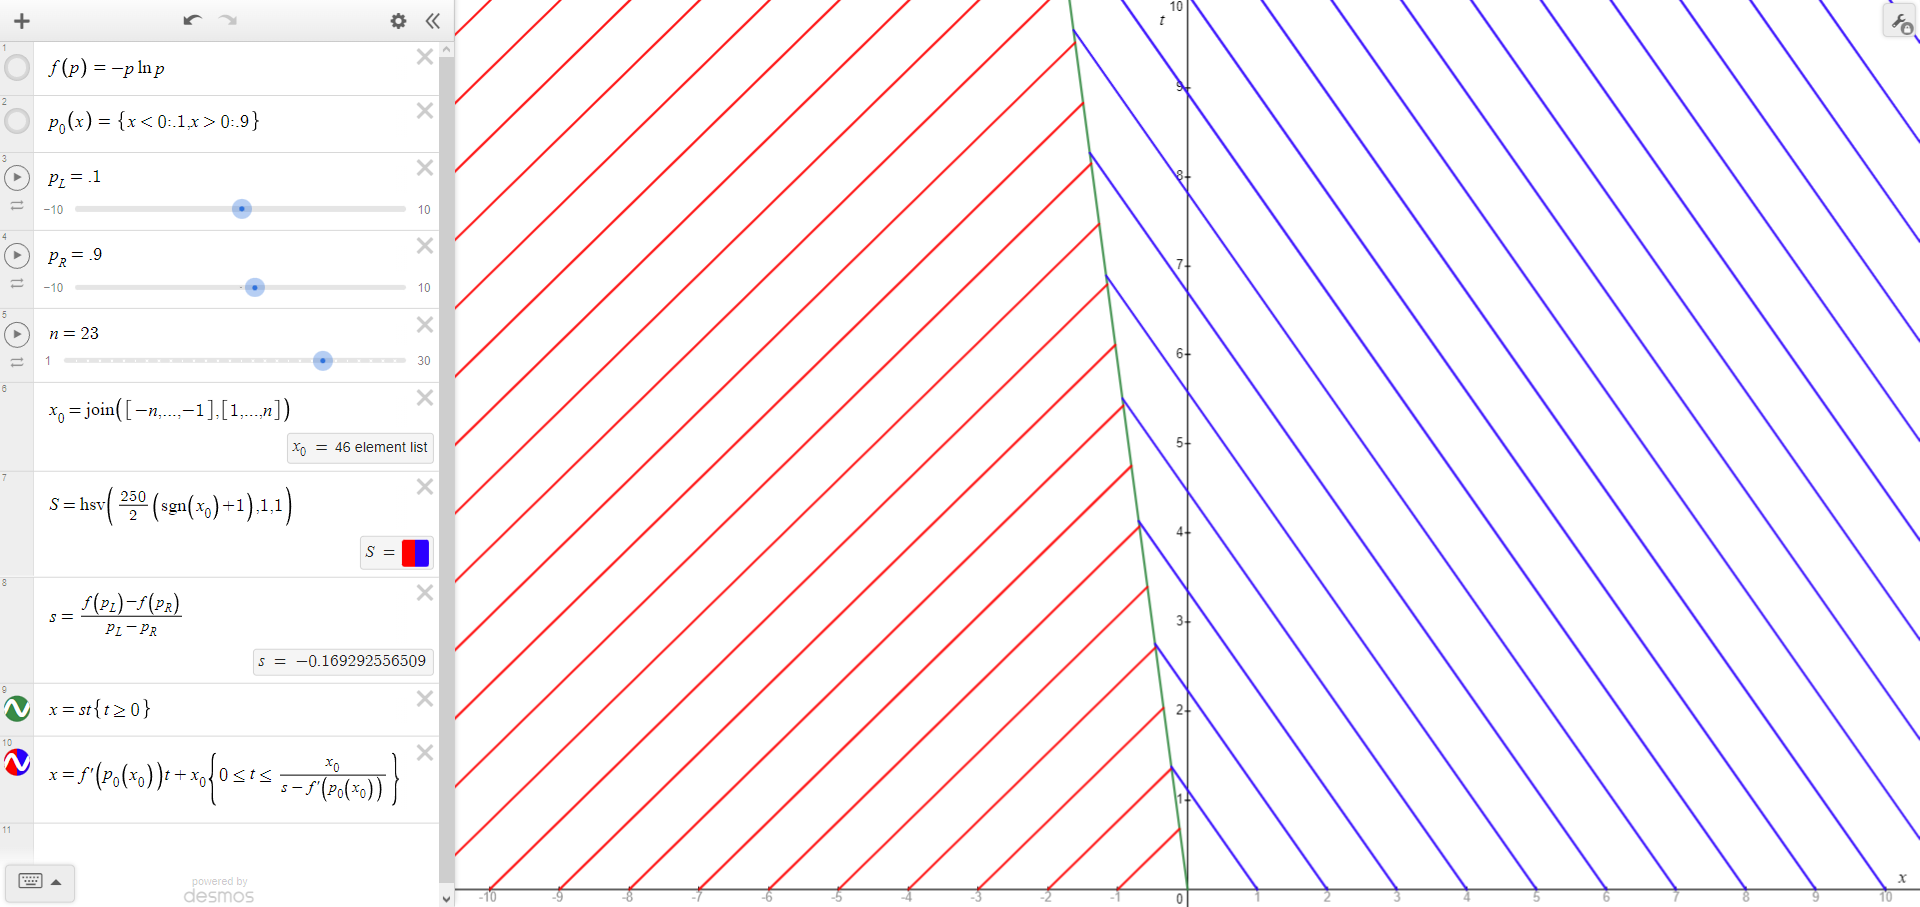
\includegraphics[scale=.3]{hw12 plot}
\end{center}


\item In this part the initial density is
$$\rho_0(x) = \frac12 + \frac{9}{10\pi}\arctan x$$
First compute
$$f''(\rho) = -\rho\inv,
\quad \rho_0'(x) = \frac{9}{10\pi}(x^2+1)\inv$$
The equation of a characteristic starting at a point $(x_0,0)$, considered as function of $t$ and $x_0$, is
$$x = f'(\rho_0(x_0))t + x_0$$
Then the shock appears at time $t_s$ when $\ptl_{x_0}x=0$, i.e.
$$f''(\rho_0(x_0))\rho_0'(x_0)t_s + 1 = 0$$
$$\imp t_s = -\sbr{f''(\rho_0(x_0))\rho_0'(x_0)}\inv
= -\sbr{-\br{\frac12 + \frac{9}{10\pi}\arctan x_0}\inv \frac{9}{10\pi}(x_0^2+1)\inv}\inv$$
$$= \br{\frac12 + \frac{9}{10\pi}\arctan x_0} \frac{10\pi}{9}(x_0^2+1)
= \br{\frac{5\pi}{9} + \arctan x_0}(x_0^2 + 1)$$
Now we find
$$\lim_{x\to\pm\infty}\rho_0(x) = \frac12 + \frac{9}{10\pi}\br{\pm\frac\pi2}
= \frac12 \pm \frac{9}{20}
\imp \rho_L = \frac{1}{20},
\quad \rho_R = \frac{19}{20}$$
Then compute
$$f(\rho_L) = -\frac{1}{20}\ln\frac{1}{20} = \frac{1}{20}\ln20$$
$$f(\rho_R) = -\frac{19}{20}\ln\frac{19}{20} = \frac{19}{20}\ln\frac{20}{19}$$
Thus the eventual shock speed is
$$s = \frac{f(\rho_L) - f(\rho_R)}{\rho_L - \rho_R}
= \frac{\frac{1}{20}\ln20 - \frac{19}{20}\ln\frac{20}{19}}{\frac{1}{20} - \frac{19}{20}}
= \frac{\ln20 - 19\ln20 + 19\ln19}{1 - 19}
= \ln20 - \frac{19}{18}\ln19
\approx -0.112$$

\end{enumerate}

\end{document}